%!TEX root = ../../../../report.tex
\subsection{Gears} % (fold)
\label{sub:gears}
The gears have been optimized based on a trade-off between manufacturability and performance.
As defined in the analysis chapter \ref{cha:analysis}, the hip will be designed without any passive actuator and the motor will be as close as possible to the joint.
This make the geared transmission the most appropriated.
When sizing the motors in \ref{cha:mathematical_model}, the same kind of motor for all the the joints was chosen reducing then the number of unique parts and increasing the modularity.
A reduction of 2:1 was needed then for the hip.

An smaller teeth size has been sought in order to reduce the backlash and assuring that there are always teeth in contact.
The size of the teeth has been defined by the smaller precision of the 3D printer in which they will be printed.

The gears have been designed with the \textit{Coarse Pitch Involute 20 deg} standard due to its easy manufacturability.
Despite a \textit{double helical} gear was considered, the simple \textit{spur} was chosen due to it easy the assembly and can be adapted to unpredicted problems in the manufacturing and assembly processes. 
In the figure \ref{fig:teeth_detail}, a detail of the teeth is shown.

\begin{figure}[ht!]
  \centering
  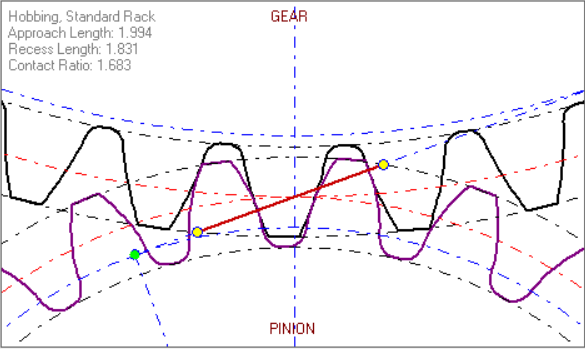
\includegraphics[width=0.5\textwidth]{figures/hip_gears}
  \caption{Teeth detail from pinion and gear.}
  \label{fig:teeth_detail}
\end{figure}

There was not a FEM or stress analysis and the experimental method was preferred due to the current unpredictable mechanical efforts of the 3D printed parts. In the appendix \ref{app:hip_gears}, all the properties of the gears are found.

% subsection gears (end)